%--------------------------INITIALISATION DU DOCUMENT---------------------%
%											%														%											%
%                        >>>> Ne pas modifier cette partie <<<<			%
																																					
\documentclass[letterpaper,12pt,oneside,final]{book}



%%
%%  Version: 2014-10-28
%%
%%  Accepte les caractères accentués dans le document (UTF-8).
\usepackage[utf8]{inputenc}
%%
%% Support pour l'anglais et le français (français par défaut).
%\usepackage[cyr]{aeguill}
\usepackage{lmodern}      % Police de caractères plus complète et généralement indistinguable visuellement de la police standard de LaTeX (Computer Modern).
\usepackage[T1]{fontenc}  % Bon encodage des caractères pour qu'Acrobat Reader reconnaisse les accents et les ligatures telles que ffi.
\usepackage[english,frenchb]{babel} % le langage par défaut est le dernier de la liste, c'est-à-dire français
%%
%% Charge le module d'affichage graphique.
\usepackage{graphicx}
\usepackage{epstopdf}  % Permet d'utiliser des .eps avec pdfLaTeX.
%%
%% Recherche des images dans les répertoires.
\graphicspath{{./images/}{./dia/}{./gnuplot/}}
%%
%% Un float peut apparaître seulement après sa définition, jamais avant.
\usepackage{flafter,placeins}
%%
%% Utilisation de natbib pour les citations et la bibliographie.
\usepackage{natbib}
%%
%% Autres packages.
\usepackage{amsmath,color,soulutf8,longtable,colortbl,setspace,ifthen,xspace,url,pdflscape,tikz,pgfplots}
%%
%% Support des acronymes.
\usepackage[nolist]{acronym}
\onehalfspacing                % Interligne 1.5.
%%
%% Définition d'un style de page avec seulement le numéro de page à
%% droite. On s'assure aussi que le style de page par défaut soit
%% d'afficher le numéro de page en haut à droite.
\usepackage{fancyhdr}
\fancypagestyle{pagenumber}{\fancyhf{}\fancyhead[R]{\thepage}}
\renewcommand\headrulewidth{0pt}
\makeatletter
\let\ps@plain=\ps@pagenumber
\makeatother
%%
%% Module qui permet la création des bookmarks dans un fichier PDF.
%\usepackage[dvipdfm]{hyperref}
\usepackage{hyperref}
\usepackage{caption}  % Hyperlien vers la figure plutôt que son titre.

\usepackage{esint}
\usepackage{geometry}
\usepackage{enumerate}




\begin{document}
%--------------------------------------------------------------------------------------%

%--------------------------PAGE DE COUVERTURE------------------------------%

% A REMPLIR PAR L'ETUDIANT: 

\newcommand\monPrenom{Nawras}		%PRENOM
\newcommand\monNom{Mohammed Amin}			%NOM
\newcommand\monMatricule{1962832}	%MATRICULE
\newcommand\monGroupe{Groupe 01}		%GROUPE

%------------------------ Ne pas modifier la ligne suivante --------------%
%\newgeometry{tmargin=2.0cm, bmargin=2.0cm, lmargin=2.25cm, rmargin=2.25cm, headsep=1.0cm}
\newgeometry{top=2cm}
\definecolor{gris1}{gray}{0.75}

\newcommand{\encadre}[1]{
\setlength\fboxsep{5mm}\setlength\fboxrule{1pt}
\begin{center}
\fcolorbox{black}{gris1}{
\begin{minipage}{0.94\textwidth}{#1}\end{minipage}}
\end{center}}

% encadre blanc
\newcommand{\boite}[1]{
\setlength\fboxsep{5mm}\setlength\fboxrule{1pt}
\begin{center}
\fcolorbox{black}{white}{
\begin{minipage}{0.5\textwidth}{#1}\end{minipage}}
\end{center}}


%\begin{document}

\thispagestyle{empty}

\encadre{
\begin{center}
\bf
{\Large \scshape 
Polytechnique Montr\'eal
\\
D\'epartement de Math\'ematiques et de G\'enie Industriel
}
\\
{\Huge
\

MTH1102D / MTH1102H - Calcul II
\\
Hiver 2022

\

Devoir 1

}
\end{center}
}

{
\centering

\vfill

\fcolorbox{black}{white}{
\begin{minipage}{0.94\linewidth}

\vspace{5mm}

{\bf \Large Nom : }\monNom \hspace{20mm} {\bf \Large Pr\'enom : }\monPrenom%\rule[-1mm]{56mm}{0.6pt}

\vspace{8mm}

{\bf \Large Matricule : }\monMatricule \hspace{20mm} {\bf \Large Groupe : }\monGroupe

%\vspace{8mm}
%
%{\bf \Large Signature: }\rule[-1mm]{126mm}{0.6pt}
%
%
%\vspace{5mm}

\end{minipage}}

\vfill

{
\renewcommand{\arraystretch}{1.5}
\begin{center}
\begin{tabular}{|c|c|c||c|} \hline
{\bf \Large Question}							& {\bf \Large Autres}			& 	{\bf \Large Bonus}	&  \\ 
{\bf \Large corrig\'ee}						& {\bf \Large  questions}	&		{\bf \Large \LaTeX}	& {\bf \Large Total} \\ \hline
\hspace{20mm}			{\Huge \strut}	& \hspace{20mm}						&		\hspace{20mm}				&\hspace{20mm} \\
\hspace{20mm}			{\Huge \strut}	& \hspace{20mm}						&		\hspace{20mm} 			& \hspace{20mm} {\Large /10} \\ \hline
\end{tabular}
\end{center}
}


\vfill
}

\restoregeometry
%\end{document}
%-------------------------------------------------------------------------%


%========================= Début des réponses ============================%


%-----------------------------QUESTION 1----------------------------------%
\section*{Question 1}


\begin{enumerate}[a)]
\item % a)
Étant donné le domaine, on le subdivise en intervales égaux en trouvant $\Delta x_i$ et $\Delta y_i$: \\ 
\begin{align*}
\Delta x_i &= \dfrac{(x-x_0)}{n} = \dfrac{(2-0)}{n} = \dfrac{2}{n} \\ \\
x_i &= \dfrac{(2-0)i}{n} = \dfrac{2i}{n} \\ \\
\Delta y_j &= \dfrac{(y-y_0)}{m} = \dfrac{(2-0)}{m} = \dfrac{2}{m} \\ \\ 
y_j &= \dfrac{(2-0)j}{m} = \dfrac{2j}{m} \\ \\
\end{align*}
Pour i = 1, 2, ..., n et j = 1, 2, ..., m.\\

Par la suite, nous pouvons déterminer l'aire de chaque sous-rectangle $\Delta A_{ij}$, qui est le produit des deux dimensions obtenus précédemment: \\ \\
\begin{align*}
\Delta A_{ij} =  \Delta x_i \cdot \Delta y_j = \dfrac{2}{n} \cdot \dfrac{2}{m} = \dfrac{4}{mn} \\
\end{align*}

Ensuite, nous devons calculer les coordonnées que nous allons utiliser pour chaque sous-rectangle. L'énoncé demande ici d'utiliser le coins inférieur gauche. Selon nos résultats précédents, chaque sous-rectangles se trouve dans un espace entre les coordonnées $(\dfrac{2i}{n}, \dfrac{2j}{m})$. Comme $n = m = 2$, nous pouvons donc trouver la liste de coordonnées possible pour côtés: \\
(0, 0); (0, 1); (0, 2); (1, 0); (1, 1); (1, 2); (2, 0); (2, 1); (2, 2) \\

Le coins inférieur gauche de chaque sous-rectangle se trouve facilement graphiquement --- (0, 0); (0, 1); (1, 0); (1, 1):
\\

\begin{center}
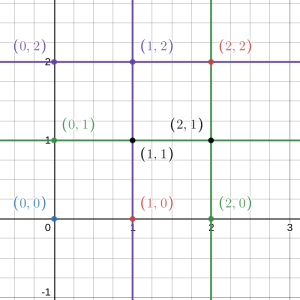
\includegraphics{graph_question1.png} \\
Figure I: Visualisation du domaine du problème ainsi que les coordonnées de chaque coins de chaque sous-rectangle.
\end{center}
\newpage
Nous sommes ensuite en mesure d'écrire équation pour l'estimation de la somme de Riemann:
\begin{align*}
 \sum_{i=1}^n\sum_{j=1}^m f(x_i^*, y_j^*) \Delta A_{ij} 
 &\approx f(0, 0) + f(0, 1) + f(1, 0) + f(1, 1) \\
 &= e^{1 -(0)^2-(0)^2} + e^{1 -(0)^2-(1)^2} + e^{1 -(1)^2-(0)^2} + e^{1 -(1)^2-(1)^2} \\
 &= e^{1} + e^{0} + e^{0} + e^{-1} \\
 &= {2 + 1/e + e} \\
 &\approx 5.0861
\end{align*}
\item % b)
Cette estimation est une sur-estimation. Ceci est dû au fait que nous avons utilisé les coins inférieurs gauches des sous-rectangles comme point d'échantillon et que la fonction à intégrée est décroissante en x et en y sur le domaine donné. Si nous repensons au calcul à une seule variable, la méthodologie équivalente consisterait à utiliser une somme de Riemann gauche, où une sous-estimation se produirait si la fonction était décroissante par rapport à sa variable indépendante. Dans notre cas, on peut prendre la dérivée partielle par rapport à x et y, si les valeurs résultantes montrent que la fonction est décroissante, alors nous avons une sur-estimation:

\begin{align*}
    \intertext{La dérivée partielle par rapport à x est: }
    &\frac{\partial f}{\partial x} = \frac{\partial \left(e^{1-x^2-y^2}\right)}{\partial x} \\
    &= -2 \cdot x \cdot e^{1-x^2-y^2} \\
    &\leq 0 \qquad \text{(Pour 0 <= x <= 2)} \\
\end{align*}
\begin{align*}
    \intertext{La dérivée partielle par rapport à y est: } \\
    &\frac{\partial f}{\partial y} = \frac{\partial \left(e^{1-x^2-y^2}\right)}{\partial y} \\
    &= -2 \cdot y \cdot e^{1-x^2-y^2} \\
    &\leq 0 \qquad \text{(Pour 0 <= y <= 2)}
\end{align*}

\end{enumerate}


%-----------------------------QUESTION 2 ---------------------------------%
\newpage \section*{Question 2}



\begin{enumerate}[a)]

\item % a)
Tout d'abord, nous devons déterminer le domaine. Comme nous savons que $y = x^2$ et que $y = 1$, nous pouvons déterminer l'intervale de x:\\
\begin{align*}
    y &= x^2 \\
    \pm \sqrt{y} &= x 
\end{align*}

Ainsi, le domaine se représente tel que $-\sqrt{y} < x < \sqrt{y}$ et $0 < y < 1$. \\

Nous pouvons maintenant résoudre l'intégrale:
\begin{align*}
&\int_0^1 \int_{-\sqrt{y}}^{\sqrt{y}} x + y + xy\cdot(x^4+y^4)^{1/5}\;dxdy \\
\end{align*}

L'intégrale d'une somme est égale à la somme d'une intégrale:
\begin{align*}
&= \int_0^1 \int_{-\sqrt{y}}^{\sqrt{y}} x \; dxdy +
\int_0^1 \int_{-\sqrt{y}}^{\sqrt{y}} y \; dxdy +
\int_0^1 \int_{-\sqrt{y}}^{\sqrt{y}} xy (x^4+y^4)^{1/5}\; dxdy \\
&= 0 + \dfrac{4}{5} + \int_0^1 \int_{-\sqrt{y}}^{\sqrt{y}} xy\cdot(x^4+y^4)^{1/5}\; dxdy \qquad \text{(Wolfram-Alpha)} \\
\end{align*}

Selon la définition d'une fonction impaire $f(-x) = -f(x)$, l'intégrande de la dernière intégrale est impaire car:

\begin{align*}
    f(-x, y) &= (-x)y\cdot((-x)^4 + y^4)^{1/5} \\
    &=-xy\cdot(x^4 + y^4)^{1/5} \\
    &= -f(x, y)
\end{align*}

Ainsi, si l'intégrande est impaire, et que son domaine est symmétrique, alors l'intégrale est nulle. Comme le domaine est $-\sqrt{y} < x < \sqrt{y}$, l'intégrale par rapport à $dx$ est nulle.

\begin{align*}
    &= 0 + \dfrac{4}{5} + \int_0^1 \int_{-\sqrt{y}}^{\sqrt{y}} xy\cdot(x^4+y^4)^{1/5}\;dxdy \\
    &= \dfrac{4}{5} + \int_0^1 0\;dy \\
    &= \dfrac{4}{5} + 0 \qquad \text{(L'intégrale définit de zéro est zéro)} \\
    &= \dfrac{4}{5}
\end{align*}

\item % b)
Avant d'essayer de résoudre l'intégrale telle quelle, puisque l'intégrande interne contient un $y^2$ qui pourrait être exclu en tant que constante si nous transformions l'intégrale en une intégrale de type 1, nous pouvons convertir l'intégrale en une intégrale de type 1.

Le domaine donné est le suivant: 

\begin{equation}
    R := {\{ (x,y) | 0 < y < 2x, 0 < x < 2\}}
\end{equation}
Nous pouvons convertir le domaine: 

\begin{align*}
    & y = 2x \\
    & \dfrac{y}{2} = x_1
\end{align*}

Avec $x_1 = \dfrac{y}{2}$ et $x_2 = 2$, nous pouvons trouver que le domaine de y est de $0 < y < 4$.

Ainsi le nouveau domaine est: 

\begin{equation}
        R := {\{ (x,y)\, |\, 0 < y < 4,\, \dfrac{y}{2} < x < 2\}}
\end{equation}

Nous pouvons ensuite résoudre l'intégrale:

\begin{align*}
   \int_0^4 \int_{y/2}^{2} y^2*e^{1+xy} \; dxdy
   &= \int_0^4 (y^2 \cdot \int_{y/2}^{2} e^{1 + xy} \; dx) dy \\
   &= \int_0^4 (y^2 \cdot \int_{y^2/2 + 1}^{2y + 1} e^{u} \; du) dy \qquad \text{(On pose u = 1 + xy; du = ydx)}  \\
\end{align*}
 Le domaine de l'intégrande est calculé à nouveau pour être conforme à la substitution:
 
 \begin{align*}
    &\rightarrow \dfrac{y}{2} \leq x \leq 2 \\
    &\rightarrow \dfrac{y^2}{2} \leq xy \leq 2y \\
    &\rightarrow \dfrac{y^2}{2} + 1 \leq xy + 1 \leq 2y + 1 \\
    &\rightarrow \dfrac{y^2}{2} + 1 \leq u \leq 2y + 1 \\
 \end{align*}
\end{enumerate}

L'intégrale se calcule donc ainsi:

\begin{align*}
   & \int_0^4 (y \cdot \int_{y^2/2 + 1}^{2y + 1} e^{u} \; du) dy \\
   &= \int_0^4 ey \cdot (e^{2y} - e^{y^2/2}) dy \qquad \text{(Wolfram-Alpha)} \\ 
   \intertext{Après factorisation application de la propriété 6 (l'intégrale d'une somme est égale à la somme des intégrales): }
  &= -e \cdot \int_0^4 ye^{y^2/2} \; dy + e \cdot \int_0^4 ye^{2y} \; dy \\
  &= -e \cdot \int_0^8 e^u \; du + e \cdot \int_0^4 ye^{2y} \; dy \qquad 
    \text{(On pose $u = 1/2 * y^2$; $du = ydy$ )} \\
  &= e -e^9 + e \cdot \int_0^4 ye^{2y} \; dy \qquad \text{(Wolfram-Alpha)} \\
  &= e -e^9 + e \cdot \int_0^4 ye^{2y} \; dy \\
  \intertext{Intégration par partie $\int fdg = fg - \int gdf$ avec $f = y, dg = e^{2y}dy$: }
  &= e - e^9 + \dfrac{1}{2}ye^{2y+1}|^4_0 - \dfrac{e}{2} \int_0^4 e^{2y} \; dy \\
  &= e + e^9 + \dfrac{1}{4}(e - e^9) \qquad \text{(Wolfram-Alpha)} \\
\end{align*}
\end{document}
